\documentclass[12pt]{beamer}
\usepackage{tikz}
\usetikzlibrary{automata}
\usetheme{EastLansing}

\begin{document}
\begin{frame}
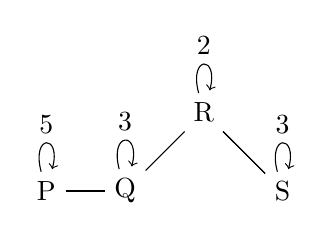
\begin{tikzpicture}
\node[](v1)at(4,1){P};
\node[](v2) at (5,1){Q};
\node[](v3) at(6,2) {R};
\node[](v4) at(7,1){S};
\draw[-](v1)--(v2);
\draw[-](v2)--(v3);
\draw[-](v3)--(v4);
\draw[-](v4)--(v3);
\draw[](v1)edge[loop above]node{5}(v1);
\draw[](v2)edge[loop above]node{3}(v2);
\draw[](v3)edge[loop above]node{2}(v3);
\draw[](v4)edge[loop above]node{3}(v4);
\end{tikzpicture}
\end{frame}
\begin{frame}

\begin{tikzpicture}
\node[](v1)at(0,0){P};
\node[](v2) at (4,1){Q};
\node[](v3) at(7,2) {R};
\node[](v4) at(8,1){S};




\draw[](v1)edge[bend left]node{2}(v2);
\draw[](v2)edge[bend left]node{1}(v3);
\draw[](v3)edge[bend left]node{1}(v4);
\draw[](v2)edge[bend left]node{4}(v1);
\draw[](v2)edge[bend right]node{6}(v4);

\end{tikzpicture}

\end{frame}
\begin{frame}[t]{Power of Digraph}
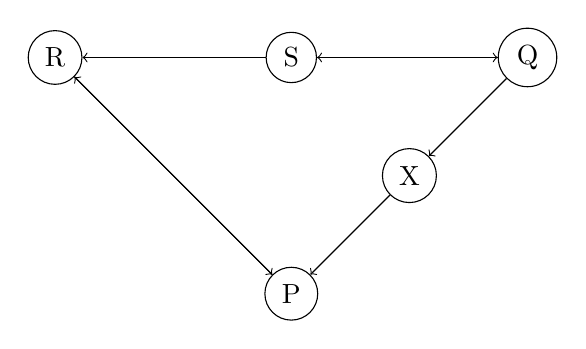
\begin{tikzpicture}
\node[circle,draw = black](v1)at(0,0){P};
\node[circle,draw = black](v2) at (3,3){Q};
\node[circle,draw = black](v3) at(-3,3) {R};
\node[circle,draw = black](v4) at(0,3){S};
\node[circle,draw = black](v5) at(1.5,1.5){X};
\draw[->](v1)--(v3);
\draw[->](v2)--(v4);
\draw[->](v2)--(v5);
\draw[->](v3)--(v1);
\draw[->](v4)--(v3);
\draw[->](v4)--(v2);
\draw[->](v5)--(v1);
\end{tikzpicture}
\end{frame}
\begin{frame}[t]
If we take p = 2 then we see following figure.\\
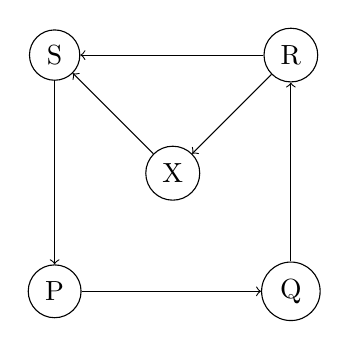
\begin{tikzpicture}
\node[circle,draw = black](v1)at(0,0){P};
\node[circle,draw = black](v2) at (3,0){Q};
\node[circle,draw = black](v3) at(3,3) {R};
\node[circle,draw = black](v4) at(0,3){S};
\node[circle,draw = black](v5) at(1.5,1.5){X};
\draw[->](v1)--(v2);
\draw[->](v2)--(v3);
\draw[->](v3)--(v4);
\draw[->](v4)--(v1);
\draw[->](v5)--(v4);
\draw[->](v3)--(v5);
\end{tikzpicture}
\end{frame}
\begin{frame}[t]{Union of Two Digraph}
Digraph H,\\
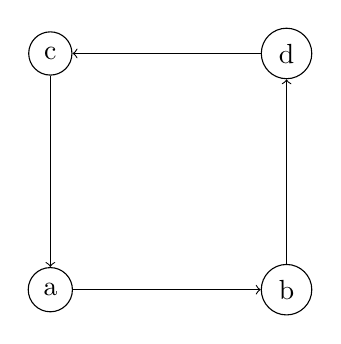
\begin{tikzpicture}
\node[circle,draw = black](v1)at(0,0){a};
\node[circle,draw = black](v2) at (3,0){b};
\node[circle,draw = black](v3) at(3,3) {d};
\node[circle,draw = black](v4) at(0,3){c};

\draw[->](v1)--(v2);
\draw[->](v2)--(v3);
\draw[->](v3)--(v4);
\draw[->](v4)--(v1);
\end{tikzpicture}
\end{frame}
\begin{frame}[t]
Digraph L.\\
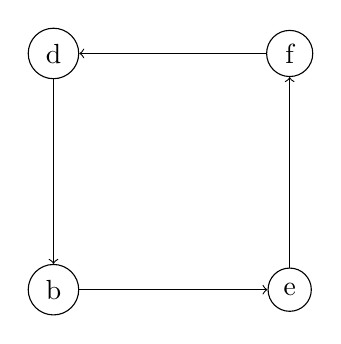
\begin{tikzpicture}
\node[circle,draw = black](v1)at(0,0){b};
\node[circle,draw = black](v2) at (3,0){e};
\node[circle,draw = black](v3) at(3,3) {f};
\node[circle,draw = black](v4) at(0,3){d};
\draw[->](v1)--(v2);
\draw[->](v2)--(v3);
\draw[->](v3)--(v4);
\draw[->](v4)--(v1);
\end{tikzpicture}
\end{frame}
\begin{frame}[t]
Union of H and L  displayed below.\\
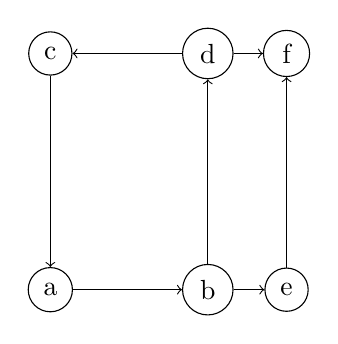
\begin{tikzpicture}
\node[circle,draw = black](v1)at(0,0){a};
\node[circle,draw = black](v2) at (2,0){b};
\node[circle,draw = black](v3) at(3,0) {e};
\node[circle,draw = black](v4) at(0,3){c};
\node[circle,draw = black](v5) at(2,3){d};
\node[circle,draw = black](v6) at(3,3){f};
\draw[->](v1)--(v2);
\draw[->](v2)--(v3);

\draw[->](v4)--(v1);
\draw[->](v2)--(v5);
\draw[->](v5)--(v4);
\draw[->](v5)--(v6);
\draw[->](v3)--(v6);
\end{tikzpicture}
\end{frame}
\end{document}